% ****** Start of file apssamp.tex ******
%
%   This file is part of the APS files in the REVTeX 4.1 distribution.
%   Version 4.1r of REVTeX, August 2010
%
%   Copyright (c) 2009, 2010 The American Physical Society.
%
%   See the REVTeX 4 README file for restrictions and more information.
%
% TeX'ing this file requires that you have AMS-LaTeX 2.0 installed
% as well as the rest of the prerequisites for REVTeX 4.1
%
% See the REVTeX 4 README file
% It also requires running BibTeX. The commands are as follows:
%
%  1)  latex apssamp.tex
%  2)  bibtex apssamp
%  3)  latex apssamp.tex
%  4)  latex apssamp.tex
%
\documentclass[%
 reprint,
superscriptaddress,
%groupedaddress,
%unsortedaddress,
%runinaddress,
%frontmatterverbose, 
%preprint,
%showpacs,preprintnumbers,
%nofootinbib,
%nobibnotes,
%bibnotes,
 amsmath,amssymb,
 aps,
%pra,
%prb,
%rmp,
%prstab,
%prstper,
%floatfix,
]{revtex4-1}

\usepackage{graphicx}% Include figure files
\usepackage{dcolumn}% Align table columns on decimal point
\usepackage{bm}% bold math
%\usepackage{hyperref}% add hypertext capabilities
%\usepackage[mathlines]{lineno}% Enable numbering of text and display math
%\linenumbers\relax % Commence numbering lines

%\usepackage[showframe,%Uncomment any one of the following lines to test 
%%scale=0.7, marginratio={1:1, 2:3}, ignoreall,% default settings
%%text={7in,10in},centering,
%%margin=1.5in,
%%total={6.5in,8.75in}, top=1.2in, left=0.9in, includefoot,
%%height=10in,a5paper,hmargin={3cm,0.8in},
%]{geometry}

\begin{document}

%\preprint{APS/123-QED}

\title{Absolute calibration of gravitational wave detector using gravity field and photon pressure}% Force line breaks with \\
%\thanks{A footnote to the article title}%
\author{Yuki Inoue}
\author{ Sadakazu Haino}
\affiliation{Institute of Physics, Academia Sinica, Taipei 11529, Taiwan}
\affiliation{High Energy Accelerator Research Organization (KEK), Ibaraki 305-0801, Japan}

\author{Nobuyuki Kanda}
\affiliation{Department of Physics, Graduate School of Science, Osaka City University, Osaka 558-8585, Japan}
\author{Yujiro Ogawa}
\affiliation{High Energy Accelerator Research Organization (KEK), Ibaraki 305-0801, Japan}
\affiliation{The Graduate University for Advanced Studies), Hayama, Miura District, Kanagawa 240-0115, Japan}
\author{Toshikazu Suzuki}
\affiliation{High Energy Accelerator Research Organization (KEK), Ibaraki 305-0801, Japan}
\affiliation{Kavli Institute for the Physics and Mathematics of the Universe (Kavli IPMU), The University of Tokyo, Chiba 277-8568, Japan}
\affiliation{Institute for Cosmic Ray Research, The University of Tokyo, Chiba 277-8582, Japan}
\author{Takayuki Tomaru}
\affiliation{High Energy Accelerator Research Organization (KEK), Ibaraki 305-0801, Japan}
\affiliation{The Graduate University for Advanced Studies), Hayama, Miura District, Kanagawa 240-0115, Japan}
\affiliation{Kavli Institute for the Physics and Mathematics of the Universe (Kavli IPMU), The University of Tokyo, Chiba 277-8568, Japan}
\affiliation{Institute for Cosmic Ray Research, The University of Tokyo, Chiba 277-8582, Japan}
\author{Takahiro Yamanmoto}
\affiliation{Institute for Cosmic Ray Research, The University of Tokyo, Gifu 506-1205, Japan}
\author{Takaaki Yokozawa}
\affiliation{Institute for Cosmic Ray Research, The University of Tokyo, Gifu 506-1205, Japan}
%\affiliation{High Energy Accelerator Research Organization (KEK), Ibaraki 305-0801, Japan}

%, Nobuyuki Kanda\supit{c}, Yujiro Ogawa\supit{b,d}, Toshikazu Suzuki\supit{b,e,f}, Takayuki Tomaru\supit{b,d,e,f}, Takahiro Yamamoto\supit{g}, Takaaki Yokozawa\supit{g}
%\skiplinehalf
%\supit{a}Institute of Physics, Academia Sinica, Taipei 11529, Taiwan; \\
%\supit{b}High Energy Accelerator Research Organization (KEK), Ibaraki 305-0801, Japan;\\
%\supit{c}Department of Physics, Graduate School of Science, Osaka City University, Osaka 558-8585, Japan;\\
%\supit{d}SOKENDAI (The Graduate University for Advanced Studies), Hayama, Miura District, Kanagawa 240-0115, Japan;\\
%\supit{e}Institute for Cosmic Ray Research, The University of Tokyo, Chiba 277-8582, Japan;\\
%\supit{f}Kavli Institute for the Physics and Mathematics of the Universe (Kavli IPMU), The University of Tokyo, Chiba 277-8568, Japan;\\
%\supit{g}Institute for Cosmic Ray Research, The University of Tokyo, Gifu 506-1205, Japan;\\
%}

%\author{Yuki Inoue}
 %\email{iyuki@post.kek.jp}
%\affiliation{Institute of Physics, Academia Sinica, Taipei 11529, Taiwan.}
%\author{Sadakazu Haino}%
%\affiliation{Hoge}%
%\author{Nobuyuki Kanda}
%\altaffiliation[a]{Hoge}%
%\date{\today}% It is always \today, today,
             %  but any date may be explicitly specified

\begin{abstract}
Absolute calibration of the gravitational wave detectors is an essential to evaluate the various parameters of the gravitational wave sources. 
The photon calibrator is the primary calibrator for the absolute calibration of the mirror displacement by using the photon pressure. 
The current technological limit of the absolute calibration uncertainty is a few~\%, corresponding to the uncertainty of the laser power standard of the standard metrology institutes from nine countries.  In order to reduce the uncertainty of the photon calibrator, we propose a new method using the combination of photon calibrator and gravity field calibrator. The gravity field calibrator gives the modulation to mirror using the gravity gradient. In previous studies, uncertainty of the distance between the test mass and the gravity field calibrator is one of the serious systematic errors of the absolute calibration. To cancel this uncertainty, we newly propose the method of quadrupole and hexapole mass distribution.  We also estimated the uncertainty of this method. The estimated precision of absolute calibration is 0.17~\%, which is 10 times less than that of previous method.
\end{abstract}

\pacs{Valid PACS appear here}% PACS, the Physics and Astronomy
                             % Classification Scheme.
%\keywords{Suggested keywords}%Use showkeys class option if keyword
                              %display desired
\maketitle

%\tableofcontents

\section{Introduction}

%Overview of GW observation
The discovery of the gravitational wave (GW) gave us the new probe for observing our universe~\cite{PhysRevLett.116.061102}. 
The typical strain sensitivity, $h$, of 2nd generation interferometric detectors (IFO), such as Advanced LIGO~\cite{0264-9381-32-7-074001}, Advanced Virgo~\cite{0264-9381-32-2-024001}, and KAGRA~\cite{0264-9381-29-12-124007, PhysRevD.88.043007}, are around $10^{-23}/\sqrt{\mathrm{Hz}}$ at 100 Hz. 
% Added by SH 180412
By using the GW signals from compact binary coalescences, we can derive 
the parameters such as masses, spins, luminosity distance, orbital inclination 
and the sky location of the binary system from the detected waveforms. 
The precision of the derived parameters are potentially limited by the 
calibration accuracy. As the number of detected sources increases and we 
detect the higher signal-to-noise ratio (SNR) events, the calibration uncertainty 
will become the dominant source of the errors to extract physics information. 
In particular, the uncertainty on the absolute GW signal amplitude directly 
propagates to the error in the estimation of the distance to the sources. 
The detection of GW signal from a Binary Neutron Star (BNS) system, 
GW170817~\cite{GW170817:2017aa} in both GW and Electromagnetic (EM) 
waves opened a new era of multi-messenger astronomy. These observations 
allow us to use GW170817 as a standard 
siren~\cite{Abbott:2017xzu,Schutz_1986,Holz_2005,Nissanke_2010} to 
determine the absolute luminosity distance to the source directly from the 
GW signal measurements. Assuming the event rate of 3000 Gpc$^{-3}$yr$^{-1}$ 
which is consistent with the bounds from GW170817 at 90~\% 
confidence~\cite{GW170817:2017aa}, we expect to detect GW signals from about 
50 BNS standard sirens in the next few observing runs. 
They can constrain the Hubble constant ($H_0$) 
measurement to 2~\% or less~\cite{Feeney:2018mkj}, and eventually resolve 
the 3-$\sigma$ tension of the $H_0$ measurement between Cephied-SN distance 
ladder~\cite{Riess_2016} and CMB data assuming a $\Lambda$CDM 
model.~\cite{2016-planck} The systematic errors in the calibration of 
the absolute GW signal amplitude must be suppressed at the sub-\% level to 
achieve higher precision $H_0$ measurement with the GW standard sirens.

% Commented out by SH 180412
%In order to estimate the parameters of gravitational waves, such as masses, spins, redshift and distance, understanding of the systematic and statistical noise sources are critical.
%In particular, the uncertainty of the absolute calibration directly propagate to the estimation error of the distance of the GW sources. The multi messenger observations of the binary neutron star, GW170817, open the new method to estimate the Hubble constant. The accuracy of estimation of the constant is proportional to the systematic uncertainties of source distance. 
% Commented out by SH 180412

%To understand the origin of heavier binary black hole, we need to obtain the precise mass and distance distribution. So, the improvement of absolute calibration is one of the important topic for the future gravitational wave astronomy.

%Calibration
An interferometer measures the change of distance difference along the two arms of the interferometer. Then, the fluctuations in the degree of freedom of differential arm length (DARM) is suppressed by the DARM control loop. The reconstruction signal of DARM fluctuation at the observation frequency is excited by the gravitational waves. We can reconstruct the gravitational waveform with the calibrated error and control signals of this DARM loop. To calibrate the signals, the accurate modelings of the actuator and sensing function are essential. To understand the model, we need to measure the transfer function and monitor the time dependency of the transfer function using continuous sine curves (calibration lines). The residual of the time-dependent model corresponds to uncertainty of the detection.

%Pcal
To reduce the calibration systematic uncertainty, we need to inject well parameterized calibration line by the photon calibrator (Pcal) or other calibration source for monitoring the time variation of the response of the IFO. The technology of Pcal was established by the Glasgow and GEO600~\cite{CLUBLEY200185,MOSSAVI20061}. Advanced LIGO improved the Pcals for the calibration of time-dependent response of IFO~\cite{0264-9381-32-2-024001, doi:10.1063/1.4967303,0264-9381-27-8-084024,0264-9381-26-24-245011,0264-9381-32-2-024001}. However, it has a challenging issue of the absolute calibration due to the accuracy of the absolute laser power of laser standard between national metrology institute from nine countries~\cite{EUROMET}. The valiation of the absolute power between these institutes is about a few \% \footnote{Figure. 9 at page 46. from \cite{EUROMET} shows the absolute power measurement between the standard institute from nine countries. The 
systematic discrepancies between nine countries are as large as 3.5 \%.}.

%KAGRA and Our approach
The gravity field calibrator (Gcal) is one of the candidates to be able to solve the uncertainty problem of absolute calibration. The technologies of the system are established and tested in Forward and Miller~\cite{doi:10.1063/1.1709366}, Weber~\cite{PhysRevLett.18.795,PhysRev.167.1145}, University of Tokyo~\cite{Hirakawa,1347-4065-19-3-L123,1347-4065-20-7-L498,PhysRevD.26.729,PhysRevD.32.342} and Rome university group~\cite{Astone1991}. Related techniques using the Gcal for the calibration are discussed in Matone et al \cite{0264-9381-24-9-005}. It can modulate the test mass using gravity gradient with rotor. The amplitude of displacement of the mirror is determined by masses, distance, frequency, radius, and gravity constant. 
%Chap1 is XXXXX, … .

In this paper, we propose how we can achieve sub-percent uncertainty of the calibration. We focus on the combination method of the Pcal and Gcal.
In section~\ref{sec:Pcal}, we explain how to calibrate with Pcal. In chapter~\ref{sec:Gcal}, we show the principle of multipole moment gravity and modulation method.
In section \ref{sec:PGCAL}, we show how to calibrate the absolute displacement with Pcal and Gcal. In section~\ref{sec:EST}, we discuss the systematic error by changing operation parameters and estimate the current technological limit using typical assumptions. 

\section{Photon calibrator} \label{sec:Pcal}
Pcal relies on the photon radiation pressure from the power modulated laser beams reflecting on the test mass to apply periodic force via the recoil of photons~\cite{doi:10.1063/1.4967303}. 
Advanced LIGO, Advanced Virgo and KAGRA employ the Pcal for the calibration of the interferometer response~\cite{0264-9381-34-1-015002, KAGRA_Pcal,0264-9381-32-2-024001}. Each gravitational detector placed the 1047~nm laser around the end test mass. The displacement of the test mass can be described as
\begin{equation}
 x = \frac{P \cos{\theta}}{2c} s(\omega)\left(1+\frac{M}{I}\vec{a} \cdot \vec{b} \right) , \label{eq:pcal}
\end{equation}
where $P$ is absolute laser power, $\theta$ is the incident angle of the Pcal laser, $M$ is  mass of test mass, $\omega$ is the angular frequency of the laser power modulation, $\vec{a}$ and $\vec{b}$ are the position vectors of Pcal laser beams. The schematic view is shown in Fig.~\ref{fig:Pcal}. $I=Mh^2/12+Mr^2/4$ is the moment of inertia, where $h$ and  $r$ are thickness and radius of test mass. $s(\omega)$ is transfer function between force and displacements. We can regard the $s(\omega)$ as $1/(M \omega^2)$ above 20 Hz. 

The noise of the laser power is stabilized to be less than design sensitivity. The schematic view of the photon calibrator is shown in Fig.~\ref{fig:Pcal}. The stabilized laser is mounted on the transmitter module. The power is monitored by the response of the photo detectors at the transmitter module, $V_{\mathrm{TxPD}}$, and receiver module, $V_{\mathrm{RxPD}}$.  
The largest relative uncertainty of photon calibrator is that of laser power.
Advanced LIGO and KAGRA use the working standard to cross-calibrate the relative response of each interferometer. The relative uncertainty of  each  calibrator is 0.51 \%~\cite{doi:10.1063/1.4967303}. 
The second largest relative uncertainty is an optical efficiency of the optical path. We calibrate the injected power from the outside of the vacuum chamber. Therefore, we need to consider the optical efficiency due to the transmittance of the vacuum window and reflectance of the mirrors. The measured uncertainty of optical efficiency in Advanced LIGO is 0.37 \%. 
For the absolute calibration, the detector, so called ``Gold standard", is calibrated with the laser power standard in National Institute of Standards and Technology (NIST) in Boulder, CO~\cite{taylor:1994:GEEU}. 
 After that, the responses of ``Working standard" of Hanford, Livingston and KAGRA are calibrated by the Gold standard in the LIGO Hanford observatory. 
However, the result of the comparison between accuracies of the absolute laser powers of each institute has a few~\% uncertainty. It implies that the serious systematic error in distance estimation because the uncertainty of the absolute calibration propagate in the distance of the GW source.

\begin{figure}
\begin{center}
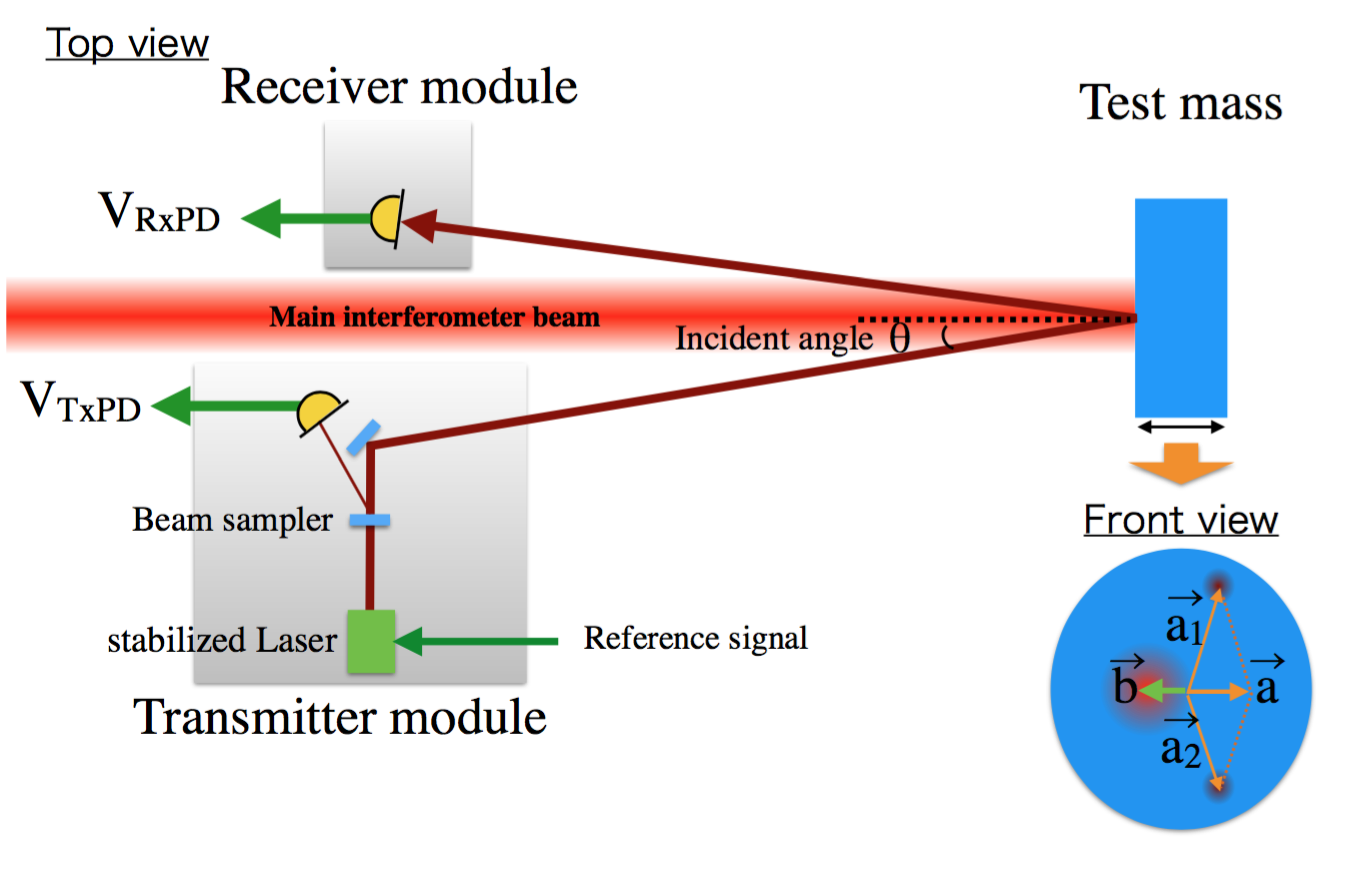
\includegraphics[width=8cm]{Pcal.eps}
\caption{Schematic view of photon calibrator. We place the stabilized laser on the transmitter module. The injected signal at the test masses is monitored by using the response of photo detector power between the transmitter module, $V_{TxPD}$ and  receiver module, $V_{RxPD}$.  The geometrical factor is characterized by the position vectors of photon calibrator beams, $\vec{a}=\vec{a_1}+\vec{a_2}$, and the main beam, $\vec{b}$.}
\label{fig:Pcal}
\end{center}
\end{figure}

\begin{table}
\begin{center}
\caption{Specification summary of Advanced LIGO, Advanced Virgo and KAGRA photon calibrator. \label{pcal}}
\footnotesize
\begin{tabular}{cccc}
\hline
& KAGRA& Advanced LIGO& Advanced Virgo \\
\hline
Mirror material & Sapphire & Silica & Silica \\
 Mirror mass & 23 kg & 40 kg & 40 kg \\
  Mirror diameter & 220 mm & 340 mm & 350 mm \\
    Mirror thickness & 150 mm & 200 mm & 200 mm \\
 Distance between Pcal & 36 m & 8 m & 1.5 m \\
and test mass &&& \\
  Pcal laser power & 20 W & 2~W & 3 W \\
  Pcal laser frequency & 1047 nm & 1047 nm &1047 nm\\
  Incident angle& 0.72 deg & 8.75 deg &30 deg \\
  \hline
\end{tabular}
\end{center}
\end{table}

\section{Gravity field calibrator} \label{sec:Gcal}
To solve the uncertainty problem of the absolute calibration, we propose the method of the gravity field calibrator. The Gcal generates the dynamic gravity field at the end of the test mass by rotating the multipole masses. The rotor placed in the vacuum chamber for isolating the acoustic noise. To monitor the frequency, we mount the 10-bit encoder. We read the response of encoder using a 16 bit analog to digital converter  system.
We calculated the displacement by changing dynamic gravity field of multipole moment with N peaces of the masses.
We assumed the suspended test mass for the interferometer and disk with multipole masses as shown in Fig ~\ref{fig:dim}.
We put the masses, $m$, at the positions of the radius, $r$. The distance between the center of mass of the mirror and the disk is assumed $d$.
We rotate the disk at the angular frequency of $\omega_{\mathrm{rot}}=2\pi f_{\mathrm{rot}}$.

\begin{figure}
\begin{center}
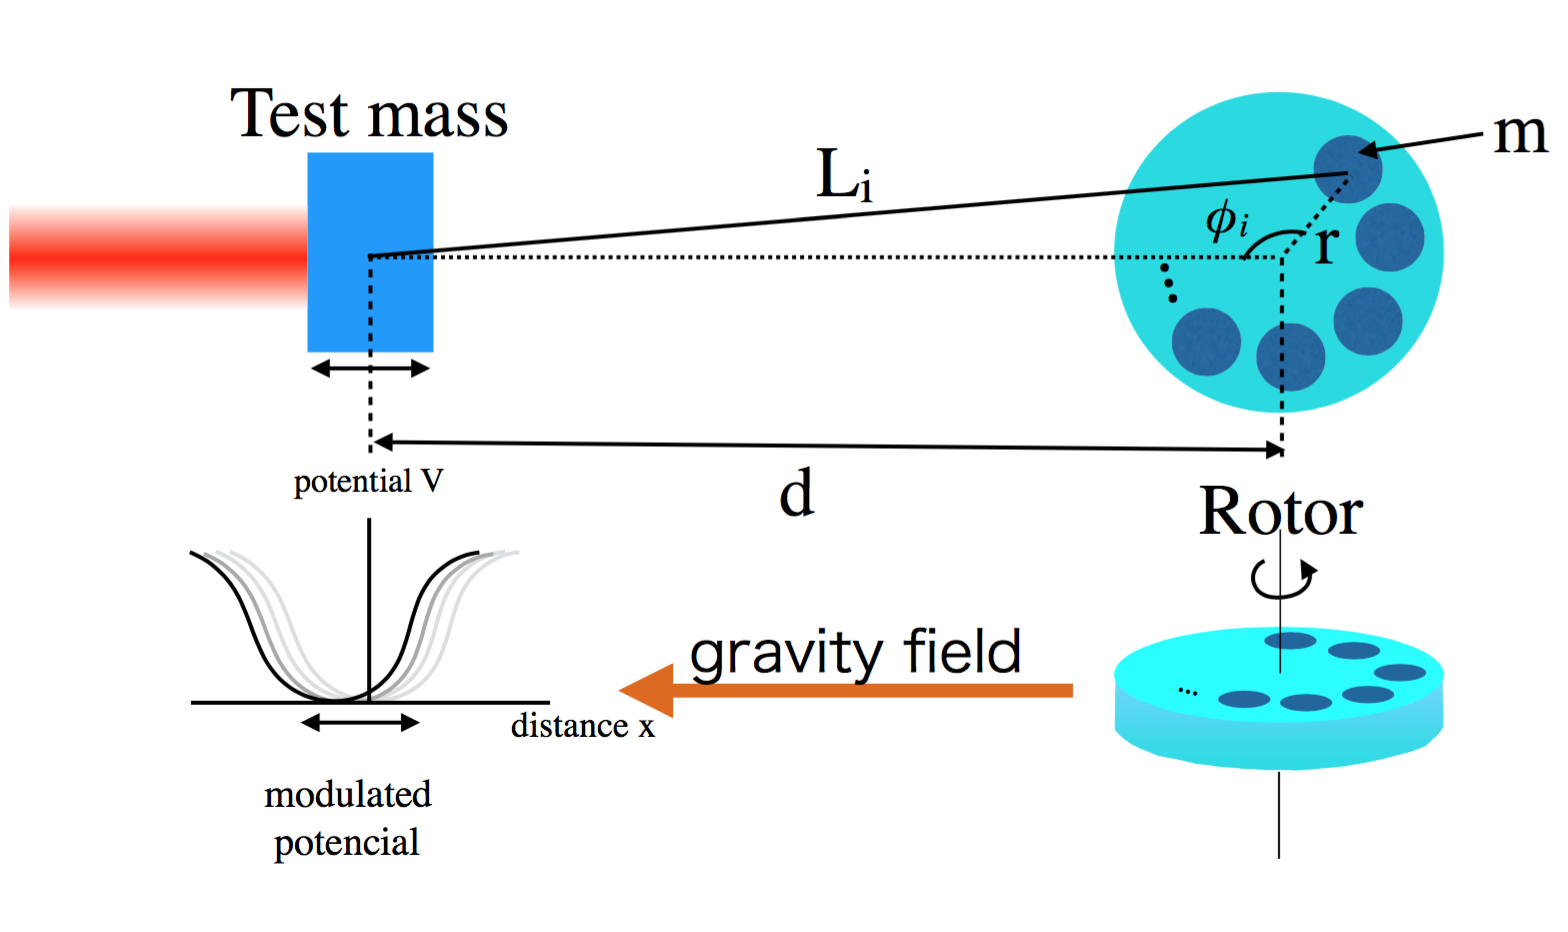
\includegraphics[width=8cm]{dim.eps}
\caption{Schematic view of Gcal. We placed the rotor at  the same height and the distance of $d$ away from test masses. Multipole mass generate the gravitational potential at the test mass position.}
\label{fig:dim}
\end{center}
\end{figure}
We estimate the equation of motion of the test mass by actuating the Gcal.
First, we calculate the distance with N pieces of masses which are separated by radius of r from the center of the rotor mass and arranged at equal intervals, respectively.
Distance between i-th mass and center of test mass is written as
\begin{equation}
L_i=d \sqrt{1+\left( \frac{r}{d} \right)^2 -2\left( \frac{r}{d} \right) \cos{\phi_i} },
\end{equation}
where the angle of i-th mass is assumed as $\phi_i=\omega_{\mathrm{rot}} t + 2\pi i/N$.
The gravitational potential at the center of test mass can be described as
\begin{eqnarray}
V &=& \Sigma^N_{i=0} V_i, \\
&=& -GMm \Sigma^N_{i=0}L_i^{-1},\\
&=&-\frac{G\!M\!m\!}{d} \Sigma^N_{i=0} \Sigma^{\infty}_{n=0}\! \left(\! \frac{r}{d}\! \right)^n
\!P_n\! \left(\! \cos{\!\left( \! \omega_{\mathrm{rot}} t \!+\!\frac{2 \pi i}{N}\right)\!}\right),
\end{eqnarray}
where $P_n$ is Legendre polynomial, and $V_i$ is potential of a mass. The equation of motion of test mass is 
\begin{eqnarray}
Ma&=&\left| \frac{\partial V}{\partial{d}} \right| =\frac{GMm}{d^2}\Sigma^N_{i=0} \Sigma^{\infty}_{n=0}(n+1) \left( \frac{r}{d} \right)^n \nonumber \\
&\times& P_n\left(\cos{\left(\omega_{\mathrm{rot}} t +\frac{2 \pi i}{N}\right)}\right),
\end{eqnarray}
where $a$ is the acceleration of test mass. 

We place the quadrupole and hexapole masses in the same rotor as shown in Fig.~\ref{fig:hex}. We put the hole between each mass. The hole can increase the gravity gradient twice effectively. Therefore, we can describe the equation of motion as 
\begin{eqnarray}
Ma&=&\left| \frac{\partial V}{\partial{d}} \right| =\frac{2GMm}{d^2}\Sigma^N_{i=0} \Sigma^{\infty}_{n=0}(n+1) \left( \frac{r}{d} \right)^n \nonumber \\
&\times& P_n\left(\cos{\left(\omega_{\mathrm{rot}} t +\frac{2 \pi i}{N}\right)}\right). \label{eq:EOM}
\end{eqnarray}
We will calculate the displacement of the quadrupole and the hexapole in the section ~\ref{Quad}  and ~\ref{Hexa}.

\begin{figure}
\begin{center}
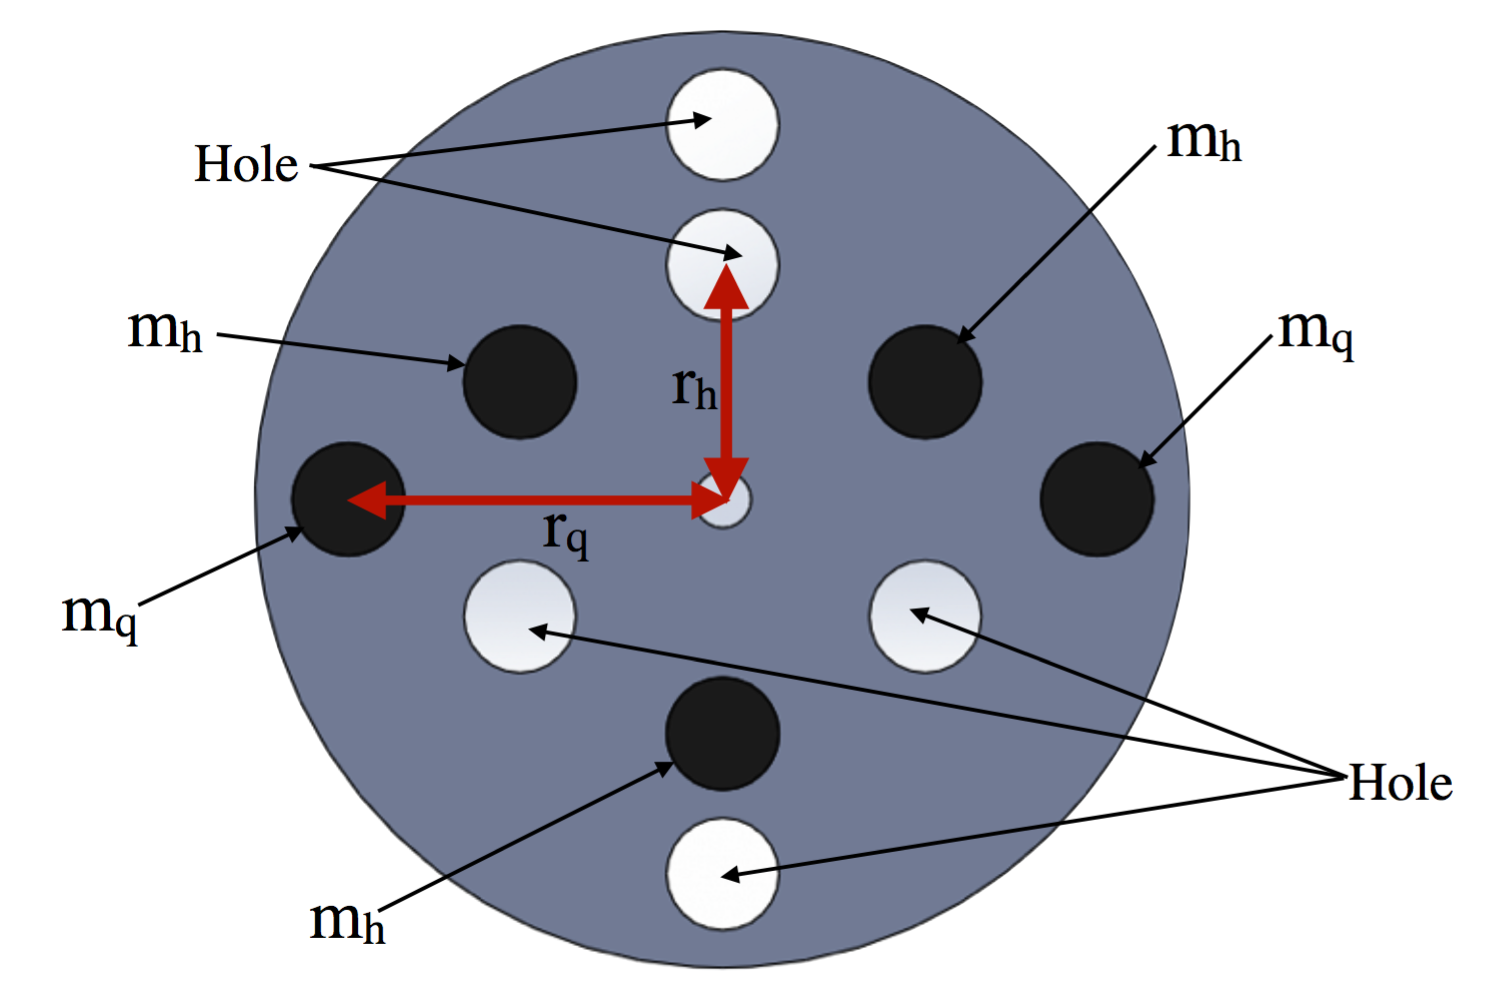
\includegraphics[width=8cm]{Hexapole.eps}
\caption{Configuration of the rotor with quadrupole and haxapole mass distributions. $m_{\mathrm{q}}$ and $m_{\mathrm{h}}$ are masses of quadrupole and hexapole. $r_{\mathrm{q}}$ and $r_{\mathrm{h}}$ are radiuses of quadrupole and hexapole.}
\label{fig:hex}
\end{center}
\end{figure}

\subsection{Displacement of test mass (Quadrupole)} \label{Quad}
We calculate the displacement of the quadrupole masses distribution corresponding to $N=2$.
The masses and radiuses of quadrupole are assumed as $m_{\mathrm{q}}$ and $r_{\mathrm{q}}$. 
The equation of motion of test mass is described as
\begin{eqnarray}
Ma&=&\frac{2GMm_{\mathrm{q}}}{d^2}\Sigma^{\infty}_{n=0}(n+1) \left( \frac{r_{\mathrm{q}}}{d} \right)^n \nonumber \\
&&\times \Sigma^1_{i=0}  P_n\left(\cos{\left(\omega_{\mathrm{rot}} t +\pi i \right)}\right).
\end{eqnarray} 
If we assume $r \ll d$, the displacement of the time-dependent lower harmonics can be written by 
\begin{equation}
x=\Sigma_{k=1}^{\infty}x_{k\mathrm{f}}\cos(k\omega_{\mathrm{rot}} t)\sim x_{\mathrm{2f}}\cos(2\omega_{\mathrm{rot}} t)=x_{\mathrm{2f}}\cos{\omega t},
\end{equation}
where $k$ is the number of the harmonics. 
The amplitude of 2-f rotation is described as
\begin{equation}
x_{2\mathrm{f}}=9\frac{GMm_{\mathrm{q}}r_{\mathrm{q}}^2}{d^4}s(\omega). \label{2f}
\end{equation}

\subsection{Displacement of test mass (Haxapole)} \label{Hexa}
We also calculate the displacement of the hexapole masses distribution, which corresponds to $N=3$.
The masses and radiuses of hexapole are assumed as $m_{\mathrm{h}}$ and $r_{\mathrm{h}}$. 
The equation of motion of test mass is described as
\begin{eqnarray}
Ma &=& \frac{2GMm_{\mathrm{h}}}{d^2}\Sigma^{\infty}_{n=0}(n+1) \left( \frac{r_{\mathrm{h}}}{d} \right)^n \nonumber \\
&&\times \Sigma^2_{i=0} P_n \left(\cos{\left(\omega_{\mathrm{rot}} t+\frac{2\pi i}{3} \right)} \right).
\end{eqnarray} 
If we assume $r \ll d$, the displacement of the time-dependent lower harmonics can be written by 
\begin{equation}
x=\Sigma_{k=1}^{\infty}x_{k\mathrm{f}}\cos(k\omega_{\mathrm{rot}} t)\sim  x_{3\mathrm{f}}\cos(3\omega_{\mathrm{rot}} t)=x_{\mathrm{3f}}\cos{\omega t},
\end{equation}
where amplitude of 3-f is described as
\begin{equation}
 x_{3\mathrm{f}}=15\frac{GMm_{\mathrm{h}}r_{\mathrm{h}}^3}{d^5}s(\omega). \label{3f}
\end{equation}

\section{Absolute power calibration by using photon calibrator and Gravity field calibrator} \label{sec:PGCAL}
In this section, we discuss about absolute laser power calibration using the interferometer. 
Figure~\ref{fig:IFO} shows the configuration of the calibration by using the combination of Pcal and Gcal.
First, we modulate the test mass using Gcal. We can measure the signal of $x_{\mathrm{2f}}$ and $x_{\mathrm{3f}}$ in the response of the interferometer. Second, we send the interferometer signal to the excitation port of photon calibrator as a reference signal port of the feedback control as shown in Fig.~\ref{fig:IFO}. The photon calibrator cancels the displacement modulated by the Gcal. Third, we measure the response of the detector of the transmitter module and the receiver module, whose units are volt. The output signal of transmitter module, $V_{\mathrm{TxPD}}$ and receiver module, $V_{\mathrm{RxPD}}$ should be corresponding to displacement from the gravity field. By using Eq~(\ref{eq:pcal}),(\ref{2f}), and (\ref{3f}), the modulated powers are
\begin{eqnarray}
 P_{\mathrm{2f}}=18 \frac{Gcm_{\mathrm{q}}Mr_{\mathrm{q}}^2}{d^4cos\theta}\frac{1}{1+\frac{M}{I}\vec{a}\cdot \vec{b}}, \label{P2f} \\
 P_{\mathrm{3f}}= 30\frac{Gcm_{\mathrm{h}}Mr_{\mathrm{h}}^3}{d^5cos\theta}\frac{1}{1+\frac{M}{I}\vec{a}\cdot \vec{b}}. \label{P3f}
\end{eqnarray}
Fourth, we demodulate the signal of the transmitter and receiver modules using the measured encoder signal of the Gcal.
The demodulated signals are 
\begin{eqnarray}
V_{\mathrm{2f}}^{\mathrm{T}}=\rho_{\mathrm{T}}P_{\mathrm{2f}}, \\
V_{\mathrm{2f}}^{\mathrm{R}}=\rho_{\mathrm{R}}P_{\mathrm{2f}}, \\
V_{\mathrm{3f}}^{\mathrm{T}}=\rho_{\mathrm{T}}P_{\mathrm{3f}}, \\
V_{\mathrm{3f}}^{\mathrm{R}}=\rho_{\mathrm{R}}P_{\mathrm{3f}}, 
\end{eqnarray} 
where $\rho_{\mathrm{T}}$ and $\rho_{\mathrm{R}}$ are the transfer functions from power to the voltage of the photo detector output at the transmitter and receiver modules.
Therefore, we can measure the distance with the ratio of response between 2-f and 3-f components: 
\begin{equation}
d=\frac{5}{3} \frac{V_{\mathrm{2f}}^{\mathrm{T}}}{V_{\mathrm{3f}}^{\mathrm{T}}}\frac{m_{\mathrm{h}}}{m_{\mathrm{q}}}\frac{r_{\mathrm{h}}^{3}}{r_{\mathrm{q}}^{2}}=\frac{5}{3} \frac{V_{\mathrm{2f}}^{\mathrm{R}}}{V_{\mathrm{3f}}^{\mathrm{R}}} \frac{m_{\mathrm{h}}}{m_{\mathrm{q}}}\frac{r_{\mathrm{h}}^{3}}{r_{\mathrm{q}}^{2}}. \label{d}
\end{equation}

Finally, we calculate the displacement formula of Pcal calibrated by Gcal. We insert the equation (\ref{2f}) to the Eq. (\ref{eq:pcal}):
\begin{eqnarray}
x&=&\frac{P \cos{\theta}}{2c} s(\omega)\left(1+\frac{M}{I}\vec{a} \cdot \vec{b} \right), \\
 &=&9\frac{Gm_{\mathrm{q}} M r_{\mathrm{q}}^2}{d^4}\frac{P}{P_{\mathrm{2f}}}s(\omega) , \\
% &=&\frac{729}{625} \frac{G m^5_q r_{\mathrm{q}}^{10}}{m^4_h r_{\mathrm{h}}^{12} \omega^2} \frac{{V_{\mathrm{3f}}^{R}}^4}{{V_{\mathrm{2f}}^{R}}^5}V^{\mathrm{R}}(\omega) .\\
 &=&\frac{729}{625} \frac{GM m^5_{\mathrm{q}} r_{\mathrm{q}}^{10}}{m^4_{\mathrm{h}} r_{\mathrm{h}}^{12} } \frac{{V_{\mathrm{3f}}^{R}}^4}{{V_{\mathrm{2f}}^{R}}^5}V_{\mathrm{in}} s(\omega)  , \label{pcal_new}
\end{eqnarray}
where we assumed $P(\omega)=\rho_{\mathrm{R}} V_{\mathrm{in}}$, and $V_{\mathrm{in}}$ is the amplitude of the input voltage.
\begin{figure}
\begin{center}
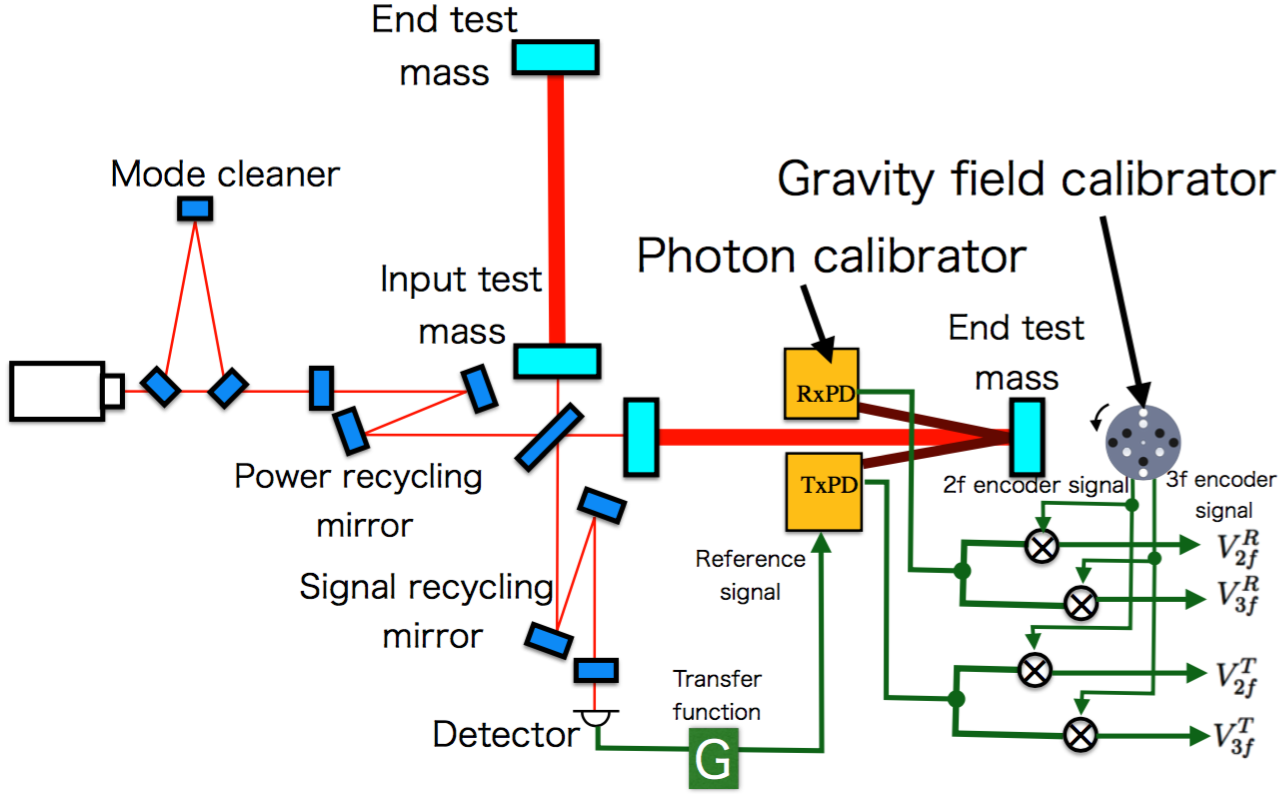
\includegraphics[width=8cm]{IFO.eps}
\caption{Test setup of the absolute calibration. We place the Gcal behind of the test mass. The frequency of the Gcal is monitored by the encoder output. The error signal of differential arm length of the interferometer sends to the reference port of the photon calibrator for canceling of the modulation of the dynamic gravity field with feedback technique, where $G$ is a transfer function. Output signals from the photon calibrator are synchronized with the force from the Gcal. We demodulate the output signals by using 2-f and 3-f signal monitored by encoder.}
\label{fig:IFO}
\end{center}
\end{figure}
The factor of $(GMm_{\mathrm{q}}^5 r_{\mathrm{q}}^{10})/(m_{\mathrm{h}}^4 r_{\mathrm{h}}^{12})$ is measurable values before the operation.  $V^R_{\mathrm{3f}}/V^R_{\mathrm{2f}}$ is measured during the calibration between Gcal and Pcal. The interval of the calibration between Pcal and Gcal depend on the power stability of the photon calibrator. In the case of Advanced LIGO, they calibrate the absolute laser power using Working standard every month. Therefor, we should operate the Gcal with same interval or less. In this method, we reconstruct the signal with photon calibrator calibrated by the Gcal.  Therefore, we do not need to operate the Gcal during the observation.
During the operation, Gcal may contaminate the noise floor by the acoustic noise and/or vibration noise. However, we can avoid this noise effect by changing the rotation frequency. We do not pay attention to the noise in the observation because we only calibrate the absolute displacement before the observation.
We consider the advantage of the demodulation. When we cancel of the modulation of Gcal with Pcal, the transfer functions of the Gcal and Pcal are also canceled. Therefore, the estimated displacement does not depend on the frequency. We can reduce the rotation systematic error with the demodulation technique.

\section{Estimation of uncertainty} \label{sec:EST}
In evaluating the accuracy of the estimated displacement, we discuss the systematic error by changing the operating frequency and distance. After that, we discuss the uncertainty of the displacement of the mirror. 
The following discussions are assumed with KAGRA basic parameters ad listed in Table~\ref{pcal} and parameters of Gcal as listed in Table~\ref{sus}. The assumed parameters of the calibrators are listed in Table~\ref{sus}. We assumed these number in the following section.

\begin{table}
\begin{center}
\caption{\label{sus}The assumed parameters. $G$ is gravity constant~\cite{RevModPhys.88.035009}. $\theta$ is incident angle of the Pcal beams. $M$ is mass of test mass. $1+\frac{I}{M}\vec{a}\cdot \vec{b}$ is geometrical factor.}
\footnotesize
\begin{tabular}{ccc}
\hline
&Value&Relative uncertainty \\
\hline
$G$&$6.67408 \times 10^{-11}~\mathrm{m^3kg^{-1}sec^{-2}}$&0.0047 \%\\
%$c$& speed of light&$2.99792458 \times 10^8$ [m/sec]& 0\%\\
$\cos{\theta}$ &1.000& 0.07~\%\\
$M$ &22.89~kg & 0.02~\%\\
$m_{\mathrm{q}}$&4.485~kg & 0.004~\%\\
$m_{\mathrm{h}}$& 4.485~kg &0.004~\%\\
$r_{\mathrm{q}}$&0.200~m & 0.010~\%\\
$r_{\mathrm{h}}$& 0.125~m & 0.016~\%\\
$1+\frac{I}{M}\vec{a}\cdot \vec{b}$& 1&0.3~\% \\
\hline
\end{tabular}\\
\end{center}
\end{table}

\subsection{Systematic error of higher order term}
In order to achieve the precision less than 1 \%, we need to consider the operation position due to the higher order of Legendre polynomials. This is because that higher order also include the 2-f and 3-f components. The $n$-th order of the Legendre polynomial is calculated in Eq.(\ref{eq:EOM}). The effect of higher order factor is mitigated by the factor of $(r/d)^n$. Table~\ref{tab:N2} and \ref{tab:N3} show the calculated displacements of the higher order terms. To compare the higher order effect, we calculate the ratio between the Finite Element Method (FEM) and calculation by changing the r/d is shown in Fig~\ref{fig:FEM-2f} and ~\ref{fig:FEM-3f}. The results show the higher order of polynomials are less than that of systematic errors. We need to place the mirror at least 2~m away from the mirror and use the sum of the first and second order equation to reduce the systematic error. In the following calculation, we assume the distance as 2~m. 

\begin{table}
\begin{center}
\caption{The calculated quadrupole($N=2$) displacement. $n$ is order of Legendre polynomial, where $\omega=n\omega_{\mathrm{rot}}$. \label{tab:N2}}
\footnotesize
\begin{tabular}{cccccccc}
\hline
& n=1 & n=2& n=3 &n=4&n=5&n=6&n=7 \\
\hline
1-f&0&0&0&0&0&0&0 \\
2-f&0&$9 \frac{Gmr^2}{d^4\omega^2}$&0&$\frac{25}{4} \frac{Gmr^4}{d^6\omega^2}$&0&$\frac{735}{128} \frac{Gmr^6}{d^8\omega^2}$&0  \\
3-f&0&0&0&0&0&0&0\\
4-f&0&0&0&$\frac{175}{16} \frac{Gmr^4}{d^6\omega^2}$&0& $\frac{441}{64} \frac{Gmr^6}{d^8\omega^2}$&0 \\
5-f&0&0&0&0&0&0&0 \\
6-f&0&0&0&0&0&$\frac{1617}{128} \frac{Gmr^6}{d^8\omega^2}$&0  \\
\hline
\end{tabular}
\end{center}
\end{table}

\begin{table}
\begin{center}
\caption{The calculated hexapole($N=3$) displacement. $n$ is order of Legendre polynomial, where $\omega=n\omega_{\mathrm{rot}}$.  \label{tab:N3}}
\footnotesize
\begin{tabular}{cccccccc}
\hline
& n=1 & n=2& n=3 &n=4&n=5&n=6&n=7 \\
\hline
1-f&0&0&0&0&0&0&0 \\
2-f&0&0&0&0&0&0&0  \\
3-f&0&0&$15\frac{Gmr^3}{d^5\omega^2}$&0&$\frac{315}{32}\frac{Gmr^5}{d^7\omega^2}$&0& $\frac{567}{64} \frac{Gmr^7}{d^9 \omega^2}$\\
4-f&0&0&0&0&0&0&0 \\
5-f&0&0&0&0&0&0&0 \\
6-f&0&0&0&0&0&$\frac{4851}{256} \frac{Gmr^6}{d^8\omega^2}$&0  \\
\hline
\end{tabular}
\end{center}
\end{table}

\begin{figure}
\begin{center}
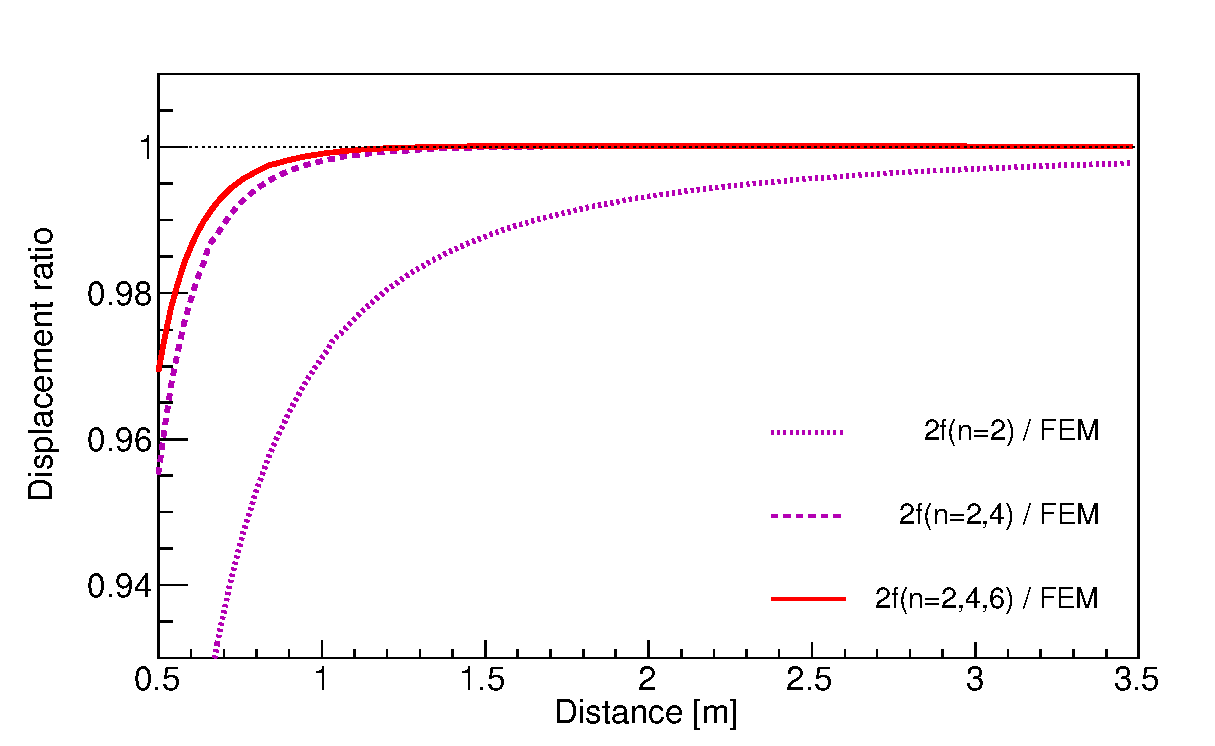
\includegraphics[width=8cm]{2f.eps}
\caption{The 2-f displacement ratio of the higher order effect by changing $r/d$. Dotted curves are included with the first order term. Dashed curves are included with sum of first order and second order. Solid Curves are assumed with sum of first, second and third order teams. The analytical result is listed in Table~\ref{tab:N2}. To achieve the precision less than 1~\%, we need to include the higher order terms.}
\label{fig:FEM-2f}
\end{center}
\end{figure}

\begin{figure}
\begin{center}
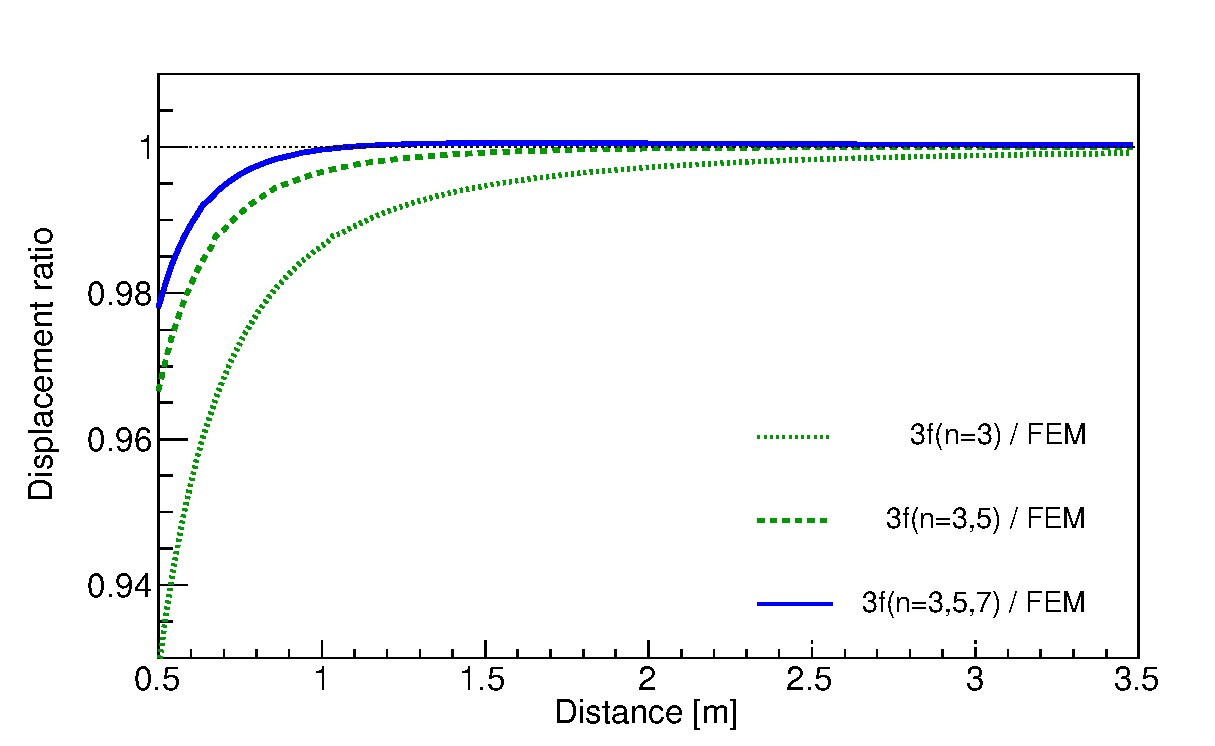
\includegraphics[width=8cm]{3f.eps}
\caption{The 3-f displacement ratio of the higher order effect by changing $r/d$. Same as Fig.~\ref{fig:FEM-2f} except for assuming Table~\ref{tab:N3}. }
\label{fig:FEM-3f}
\end{center}
\end{figure}


\subsection{Systematic error of the transfer function}
The Gcal can modulate the mirrors with gradient of gravitational potential. However, its gravity gradient acts the masses of suspension system as shown in Fig.~\ref{fig:cryo}. We simulated the transfer function by assuming the cryogenic suspension system in KAGRA~\cite{0264-9381-34-22-225001}.The transfer function is calculated by the suspension rigid-body simulation code, called SUMCON~\cite{SUMCON}. We estimated the total displacement by including all the masses. Figure \ref{fig:ratio} shows the displacement ratio between the sensed motion and the free mass motion as a function of frequency. The simulation result is in good agreement with free mass motion at the frequency larger than 20~Hz. The structures of low frequency are corresponding to the resonant peak of the suspension system. Therefore, we can neglect the intermediate mass effect and regard as free mass motion larger than 20~Hz. 
%On the other hand, we need to consider the elastic deformation~\cite{}. The effect of elastic deformation changes the shape of the mirror and transfer function between the force and displacement due to the mirror position and frequency. However, Gcal dose not generate the elastic deformation because the gravity field act the force to elements mass of the bulk of the test mass uniformly. When we estimate the distance, the difference of  the transfer function of Pcal at the 2-f and 3-f generate the systematic error. The estimated displacement ratio is shown as \ref{fig:ED}, where we assumed Pcal beam position on the mirror is XXXX mm from the center of the mirror surface.
Therefore, we need to operate the rotor larger than 20 Hz for reducing the error less than 0.1~\%.
We assumed the rotation frequency as 16~Hz, which is corresponding to 32~Hz and 48~Hz at the operating frequency of 2-f and 3-f components.  We used this assumption in the following section.

%\begin{figure}
%\begin{center}
%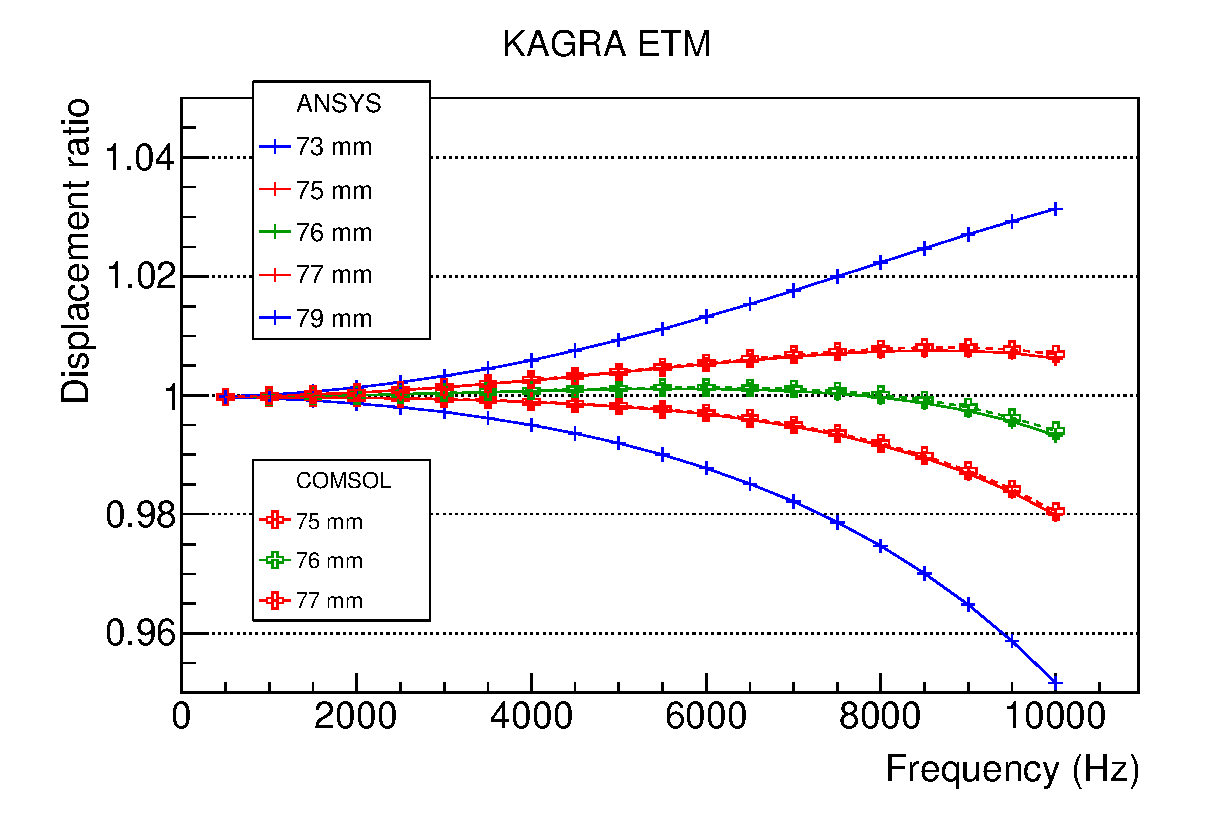
\includegraphics[width=8cm]{fem-kge-opt.eps}
%\caption{Estimated elastic deformation of the photon calibrator.}
%\label{fig:ED}
%\end{center}
%\end{figure}

\begin{figure}
\begin{center}
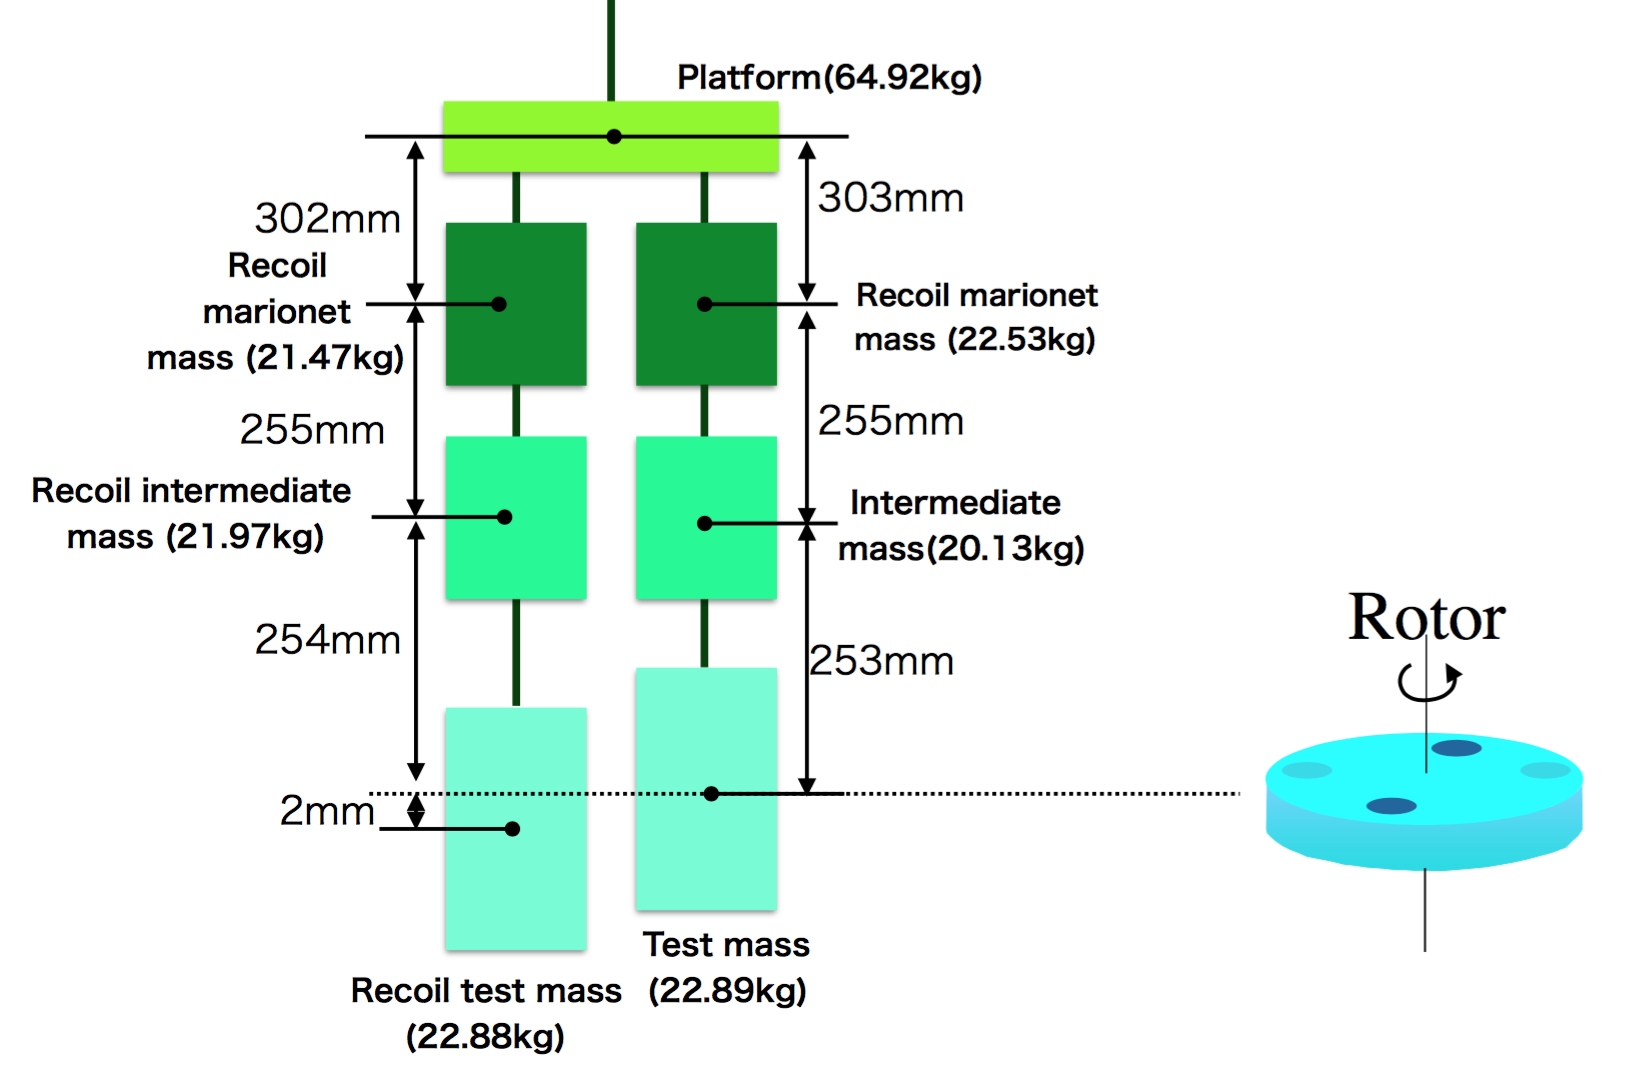
\includegraphics[width=8cm]{Cryo.eps}
\caption{Schematic view of the suspension system. The parameters of the heights and masses are the assumed values. }
\label{fig:cryo}
\end{center}
\end{figure}

\begin{figure}
\begin{center}
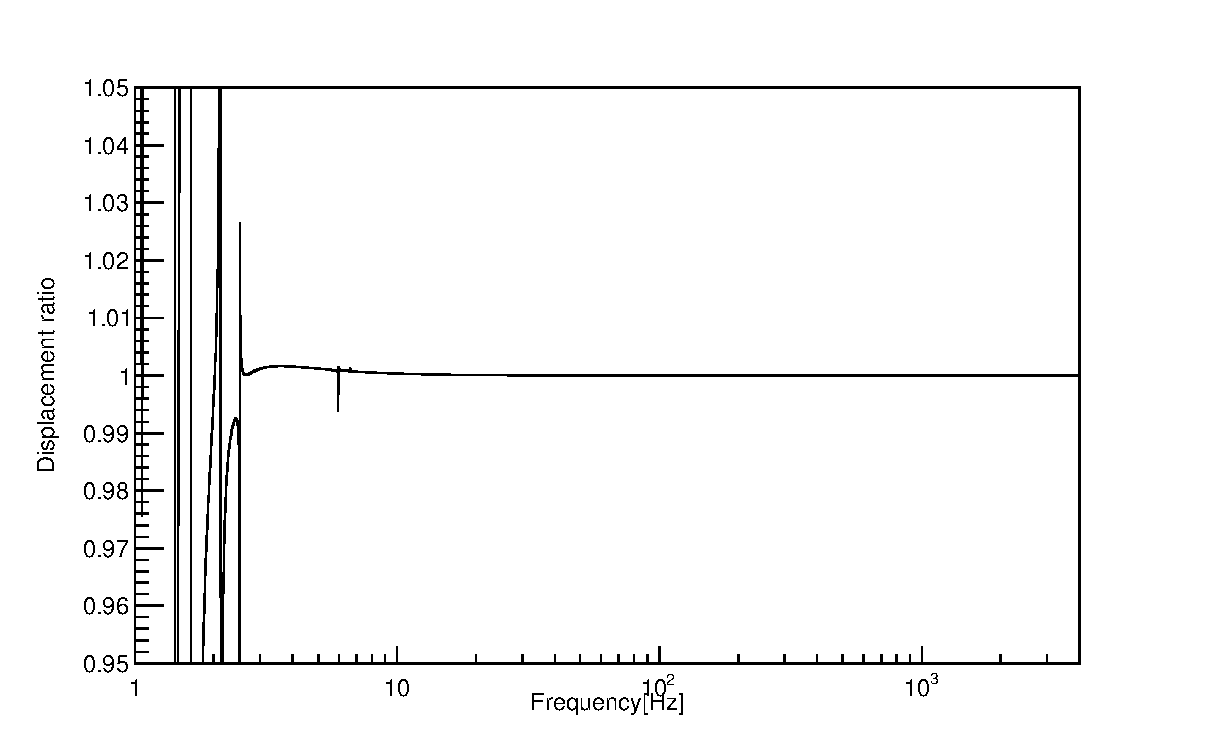
\includegraphics[width=8cm]{dx_Gcal_ratio.eps}
\caption{The displacement ratio of the transfer function of multi pendulum by changing modulation frequency, where relations of the modulation frequency, $f$, modulation angular frequency, $\omega$, and rotation angular frequency, $\omega_{\mathrm{rot}}$ are described as. $n\omega_{\mathrm{rot}}=\omega=2\pi f$. If we put the Gcal, it act the upper masses and it makes systematic error of the transfer function.}
\label{fig:ratio}
\end{center}
\end{figure}

\subsection{Uncertainty of displacement and  laser power}
In this section, we estimate the typical displacement based on the Table.~\ref{sus}. We neglect above the second order Legendre polynomial in the following discussion to simplify the discussion. 
 The estimated displacements of 2-f and 3-f are described as
 \footnotesize
\begin{eqnarray}
x^{\mathrm{rms}}_{\mathrm{2f}}&=&1.18 \times 10^{-16}\mathrm{[m]} \times \left( \frac{G}{6.67408 \times 10^{-11} \mathrm{[m^3kg^{-1}sec^{-2}]}} \right) \nonumber \\
&\times&\! \left( \! \frac{m_{\mathrm{q}}}{4.485 \mathrm{[kg]}} \!\right) \! \times \!\left( \!\frac{r_{\mathrm{q}}}{0.200 \mathrm{[m]}} \! \right)^2 \! \times \! \left( \! \frac{2\mathrm{[m]}}{d} \! \right)^4 \! \times \! \left( \! \frac{2\pi \! \times \! 32\mathrm{[Hz]}}{\omega} \! \right)^2,\\
x^{\mathrm{rms}}_{\mathrm{3f}}&=&2.13 \times 10^{-18}\mathrm{[m]} \times \left( \frac{G}{6.6742 \times 10^{-11} \mathrm{[m^3kg^{-1}sec^{-2}]}} \right) \nonumber \\
&\times& \! \left( \! \frac{m_{\mathrm{h}}}{4.485 \mathrm{[kg]}}\! \right) \! \times \! \left(  \!\frac{r_{\mathrm{h}}}{0.125 \mathrm{[m]}} \! \right)^3 
\! \times \! \left(\! \frac{2\mathrm{[m]}}{d} \! \right)^5 \! \times \! \left( \! \frac{2\pi\!\times \! 48\mathrm{[Hz]}}{\omega} \! \right)^2.
\end{eqnarray}
\normalsize

We define the signal-to-noise ratio (SNR) with the ratio of RMS displacement of the design noise spectrum density for the IFO of KAGRA at 32~Hz for 2-f and 48~Hz for 3-f.
By using this result, we estimate the SNR of the peaks.

\footnotesize
\begin{eqnarray}
\!S\!N\!R_{\mathrm{2f}}&=&392 \times \left(\frac{3.0 \times 10^{-19} [\mathrm{m/\sqrt{Hz}}]}{n_{\mathrm{32Hz}}} \right)  \times \left(\frac{T}{1 [\mathrm{sec}]} \right)^{\frac{1}{2}} \nonumber \\
 &&\times \left(\frac{x_{\mathrm{2f}}^{\mathrm{rms}}}{1.178 \times 10^{-16}\mathrm{[m]} }  \right),   \\
\!S\!N\!R_{\mathrm{3f}}&=&73 \times \left(\frac{2.9 \times 10^{-20} [\mathrm{m/\sqrt{Hz}}]}{n_{\mathrm{48Hz}}} \right) \times \left(\frac{T}{1 [\mathrm{sec}]} \right)^{\frac{1}{2}}  \nonumber \\ 
&&\times \left(\frac{x_{\mathrm{2f}}^{\mathrm{rms}}}{2.130 \times 10^{-18}\mathrm{[m] }} \right),
\end{eqnarray}
\normalsize
where $T$ is integration time. When we integrate the signal larger than 3 min, we can measure the $V^{\mathrm{R}}_{2f}$ and $V^{\mathrm{R}}_{3f}$ with SNR large enough such that systematic error can be reduced less than 0.1~\%. 
This method is applicable to the measurement of the absolute laser power. The estimated powers are
\footnotesize
\begin{eqnarray}
P_{\mathrm{2f}}&=&0.093 ~\mathrm{[W]}\times \left( \frac{G}{6.6742 \times 10^{-11} \mathrm{[m^3kg^{-1}sec^{-2}]}} \right) \nonumber \\
&& \times \left( \frac{m_{\mathrm{q}}}{4.485 \mathrm{[kg]}} \right) \times \left( \frac{r_{\mathrm{q}}}{0.200 \mathrm{[m]}} \right)^2 \times \left( \frac{2\mathrm{[m]}}{d} \right)^4 \nonumber \\ &&\times \left( \frac{1}{\cos{\theta}} \right) \times \left( \frac{1}{1+\frac{M}{I}\vec{a}\cdot \vec{b}} \right)^2,\\
P_{\mathrm{3f}}&=&0.0038~\mathrm{[W]} \times \left( \frac{G}{6.6742 \times 10^{-11} \mathrm{[m^3kg^{-1}sec^{-2}]}} \right) \nonumber \\
&& \times \left( \frac{m_{\mathrm{h}}}{4.485 \mathrm{[kg]}} \right) \times \left( \frac{r_{\mathrm{h}}}{0.125 \mathrm{[m]}} \right)^3 \times \left( \frac{2\mathrm{[m]}}{d} \right)^5 \nonumber \\ &&\times \left( \frac{1}{\cos{\theta}} \right) \times \left( \frac{1}{1+\frac{M}{I}\vec{a}\cdot \vec{b}} \right)^2.
\end{eqnarray}
\normalsize
The estimated $V^{\mathrm{T}}_{\mathrm{2f}}/V^{T}_{\mathrm{3f}}$ by changing distance are shown in Fig.~\ref{fig:dvsVV}.
\begin{figure}
\begin{center}
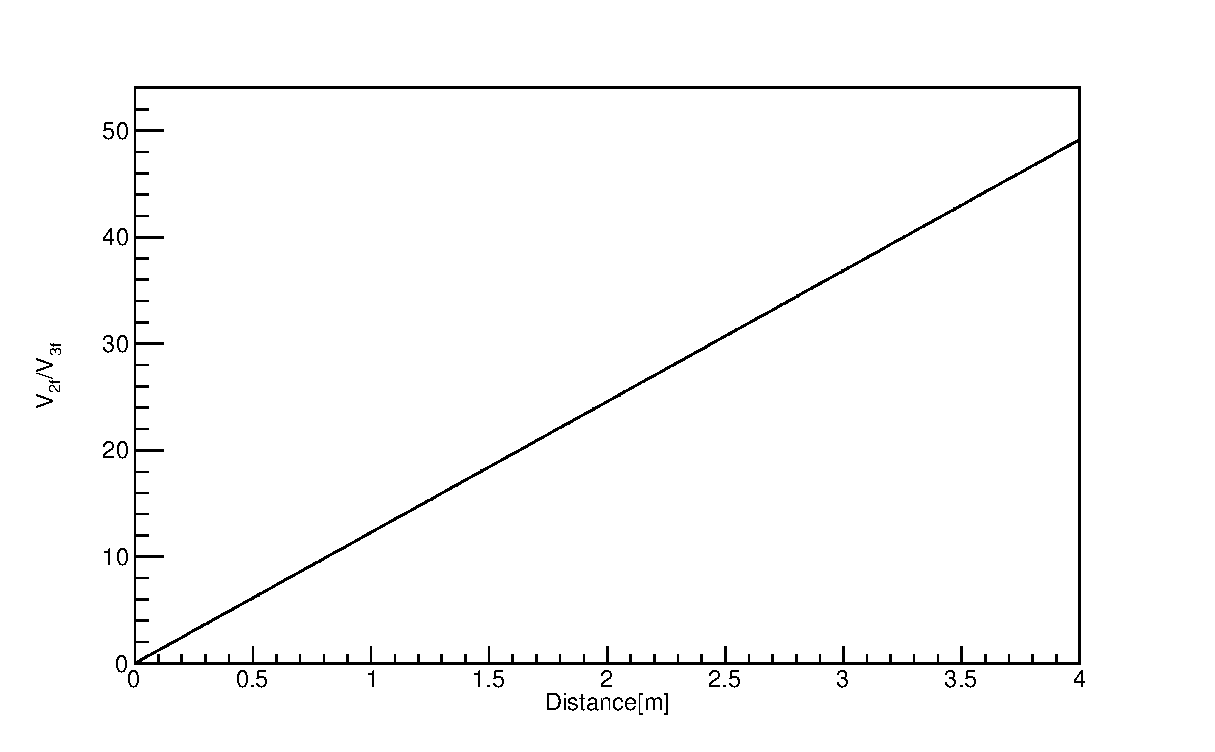
\includegraphics[width=8cm]{dvsVV.eps}
\caption{The response of $V_{\mathrm{2f}}/V_{\mathrm{3f}}$ by changing distance between test mass and Gcal.}
\label{fig:dvsVV}
\end{center}
\end{figure}
We  estimate the laser power by using the following equations:
\footnotesize
\begin{eqnarray}
\left( \frac{\delta P_{\mathrm{2f}}}{P_{\mathrm{2f}}} \right)^2 &\sim&  \!16 \! \left( \frac{\delta V^{\mathrm{R}}_{{\mathrm{2f}}}}{V^{\mathrm{R}}_{{\mathrm{2f}}}} \!\right)^2+16\left( \frac{\delta V^{\mathrm{R}}_{{\mathrm{3f}}}}{V^{\mathrm{R}}_{{\mathrm{3f}}}} \right)^2 +\left( \frac{\delta P_{\mathrm{sys}}}{P_{\mathrm{sys}}} \right)^2, \label{dP2f} \\ 
\left( \frac{\delta P_{\mathrm{3f}}}{P_{\mathrm{3f}}} \right)^2 &\sim&  \!16 \! \left( \frac{\delta V^{\mathrm{R}}_{{\mathrm{2f}}}}{V^{\mathrm{R}}_{{\mathrm{2f}}}} \right)^2+16\left( \frac{\delta V^{\mathrm{R}}_{{\mathrm{3f}}}}{V^{\mathrm{R}}_{{\mathrm{3f}}}} \right)^2+\left( \frac{\delta P_{\mathrm{sys}}}{P_{\mathrm{sys}}} \right)^2,  \label{dP3f}
\end{eqnarray}
\normalsize
where $\delta P_{\mathrm{sys}}/P_{\mathrm{sys}}$ is the relative systematic error  of the power due to the machining tolerance of the rotor masses and radiuses as disproved by
\begin{eqnarray}
\frac{\delta P_{\mathrm{sys}}}{P_{\mathrm{sys}}}&\sim& \frac{\delta G}{G} + \frac{\delta M}{M} +\frac{\delta \cos{\theta}}{\cos{\theta}}+ \frac{\delta\left( 1+\frac{M}{I}\vec{a}\cdot \vec{b} \right)}{\! \left( \! 1+\frac{M}{I}\vec{a}\cdot \vec{b} \! \right)}  \nonumber \\
&+&\frac{12}{\sqrt{6}} \frac{\delta r_{\mathrm{h}}}{r_{\mathrm{h}}} +\frac{10}{2} \frac{\delta r_{\mathrm{q}}}{r_{\mathrm{q}}}  +\frac{5}{2} \frac{\delta m_{\mathrm{q}}}{m_{\mathrm{q}}} +\!\frac{4}{\sqrt{6}}  \! \frac{\delta m_{\mathrm{h}}}{m_{\mathrm{h}}}.
\end{eqnarray}
 We consider the mitigation effect of the masses and radiuses due to the tolerance and uncertainty of the measurement instruments. The values of masses and radiuses have a variance due to the fabrication tolerance. The errors of $m_{\mathrm{q}}$, $r_{\mathrm{q}}$, $m_{\mathrm{h}}$, and $r_{\mathrm{h}}$ are mitigated by the factor of $1/\sqrt{6}$ and $1/\sqrt{4}$. 
The uncertainty of the quadrupole and hexapole masses are limited by the accuracy of  an electronic balance. In this case, we use the masses made of Tungsten. The density of Tungsten is $19.25~\mathrm{g/cm^3}$. The diameter and thickness of the mass are 0.06~m and 0.08~m, respectively. Therefore, the mass of the rotor mass is 4.485~kg. To measure this mass, we assumed that we use an electronic balance whose catalog number and accuracy are CG-6000 and 0.2~g, respectively~\cite{CG6000}. Therefore, the relative uncertainty of the mass of rotor mass is 0.04~\%.

 To make the rotor disk, we use the NC milling machine. The typical accuracy is less than 0.02 mm. For the measuring of the shape, we employ the three-dimension coordinate measuring machine (CMM)~\cite{Inoue:2016kyq}. The precision of CMM is $2~\mathrm{\mu m}$. We can measure the shape of the rotor and masses with enough of uncertainty using CMM. 

The estimated relative uncertainties of the powers are 0.52~\%. One of the largest uncertainties is the geometrical factor of the Pcal laser. The geometrical factor uncertainty is assumed 0.3 \%, which is the same number of Advanced LIGO. 

 Finally, the estimated relative uncertainty of the displacement is written as
 \footnotesize
\begin{equation}
\left( \frac{\delta x}{x} \right)^2 \!\sim \! \left( \!\frac{\delta V_{in}}{V_{in}}\! \right)^2+\left(\! \frac{\delta s(\omega)}{s(\omega)} \! \right)^2\!+\!25\!\left(\!\frac{\delta V^{\mathrm{R}}_{{\mathrm{2f}}}}{V^{\mathrm{R}}_{{\mathrm{2f}}}}\! \right)^2+16\!\left(\! \frac{\delta V^{\mathrm{R}}_{{\mathrm{3f}}}}{V^{\mathrm{R}}_{{\mathrm{3f}}}}\! \right)^2\!+ \left(\! \frac{\delta x_{\mathrm{sys}}}{x_{\mathrm{sys}}} \! \right)^2 \label{deltax},
\end{equation}
\normalsize
where $\delta x_{\mathrm{sys}}/x_{\mathrm{sys}}$ is the relative systematic error of the displacement. This factor is written by
 \footnotesize
\begin{equation}
\frac{\delta x_{\mathrm{sys}}}{x_{\mathrm{sys}}}=\frac{\delta G}{G} + \frac{\delta M}{M} +\frac{12}{\sqrt{6}} \frac{\delta r_{\mathrm{h}}}{r_{\mathrm{h}}} +\frac{10}{2} \frac{\delta r_{\mathrm{q}}}{r_{\mathrm{q}}}  +\frac{5}{2} \frac{\delta m_{\mathrm{q}}}{m_{\mathrm{q}}} +\!\frac{4}{\sqrt{6}}  \! \frac{\delta m_{\mathrm{h}}}{m_{\mathrm{h}}}.
\end{equation}
\normalsize
We assumed the mitigation factors of radiuses and masses.
To reduce the noise of the displacement, we need to reduce the uncertainty of the shape of the rotor and masses.
The uncertainty of the $V^{\mathrm{R}}_{\mathrm{2f}}$,$V^{\mathrm{R}}_{\mathrm{3f}}$, $V^{\mathrm{R}}_{0}$ are much less than that of other contributions. We can reduce the uncertainty of these values with long time integration time due to the statistics. Each the uncertainty is listed in Table.~\ref{sus}. The estimated  total uncertainty of the displacement is 0.17~\%.

% Added by SH 180414
%\begin{table}
%\begin{center}
%\caption{Comparison of systematic error contributions between eq.~\ref{deltax} and Monte Carlo simulation. \label{tab:MC}}
%\begin{tabular}{ccccc}
%\hline
%&&Relative uncertainty&Contribution(eq.~\ref{deltax})&Contribution(MC simulation)\\
%\hline
%$G$& Gravity constant&0.015 \%&0.015 \%&0.015 \%\\
%$M$& Mass of test mass& 0.02~\%& 0.02~\%& 0.02~\%\\
%$m_{\mathrm{q}}$&Mass of poles& 0.004~\% & 0.025~\% & 0.022~\%\\
%$r_{\mathrm{q}}$&Radius of poles& 0.01/0.02~\%& 0.22~\%& 0.028~\%\\
%$V^{\mathrm{R}}$&Demodulated signal& 0.001~\%& 0.006~\%& 0.006~\%\\
%\hline\hline
%$x$&displacement&& 0.22~\%& 0.048~\%\\
%\hline
%\end{tabular}\\
%\end{center}
%\end{table}
% Added by SH 180414

\section{Conclusion}
Pcal is one of the powerful calibrators in Advanced LIGO, Advanced Virgo and KAGRA. It can calibrate the response of IFO and its uncertainty is essential for the estimation of parameters of the GW source. In particular, the distance of the source strongly depends on the absolute laser power of the photon calibrator. In previous studies, the Gold standard, which response is calibrated by the laser power standard in NIST, is used for the absolute laser power calibration of the photon calibrator. However, the current limit of the absolute laser power between each country is about a few~\%. It is directly propagated to the uncertainty of the absolute displacement of the GW detector.

To solve the problem, we proposed the combination method of the photon calibrator and Gcal. The Gcal can modulate the mirror using the dynamic gravity field. By canceling the displacement of the test mass displacement using the photon calibrator, we can calibrate the absolute laser power using the Gcal.

This method has an advantage of a direct comparison of the amplitude of the injected power and gravity field. In previous studies, we need to consider the uncertainty of the optical efficiency through the window and mirrors  and geometrical factor of the laser position. This is because that we put the Working standard on the outside of the chamber. However, the method of gravity field can compare the displacement directly. By using this method, we can calibrate the uncertainty of the optical efficiency and the absolute power of the laser.  The estimated uncertainty of the power of this method is 0.52~\%. It implies that we can make a new power standard using an interferometer with 3 times improvement.

Finally, we estimate the uncertainty of the absolute calibration. The estimated absolute uncertainty of the displacement is 0.17~\%, which is 10 times better than that of previous studies. This uncertainty impact on the estimation of the distance of the gravitational wave source. Of particular importance is that the estimated uncertainty can leach the precision of the Hubble constant less than 1~\%. It may solve the tension problem between Cephied-SN distance ladder~\cite{Riess_2016} and CMB data assuming a $\Lambda$CDM 
model~\cite{2016-planck}.

\acknowledgments     %>>>> equivalent to \section*{ACKNOWLEDGMENTS}       
 
We thank Richard Savage, Darkhan Tuyrnbayev for discussion of the photon calibrator. We would like to express our gratitude to Prof. Takaaki Kajita and Prof. Henry Wong. We would like to thank the KEK Cryogenics Science Center for the support. YI and SH are supported by Academia Sinica and Ministry of Science and Technology (MOST) under Grants No. CDA-106-M06, MOST106-2628-M-007-005 and MOST106-2112-M-001-016 in Taiwan. This work was supported by JSPS KAKENHI Grant Numbers 17H106133 and 17H01135. KAGRA project is supported by MEXT, JSPS Leading-edge Research Infrastructure Program, JSPS Grant-in-Aid for Specially Promoted Research 26000005, MEXT Grant-in-Aid for Scientific Research on Innovative Areas 24103005, JSPS Core-to-Core Program, A. Advanced Research Networks, and the joint research program of the Institute for Cosmic Ray Research, University of Tokyo.

\bibliography{report}
\end{document}
%
% ****** End of file apssamp.tex ******
